\section{组合 PRG}\label{sec:3-4}

在本节中,我们将讨论两种构造,它们能让我们基于旧的 PRG 建立新的 PRG。这些构造允许我们扩展原始 PRG 的输出空间的大小,同时保证其安全性。更重要的是,在本节中,我们将介绍一种非常重要的论证技术,称为\textbf{混合论证 (hybrid argument)}。该技术在现代密码学中的应用非常广泛。

\subsection{一种并行构造}\label{subsec:3-4-1}

令 $G$ 是一个定义在 $(\mathcal S,\mathcal R)$ 上的 PRG。假设在某些应用中,我们想要多次使用 $G$。我们希望 $G$ 的所有输出都与 $\mathcal{R}$ 上的随机元素是计算上无法区分的。如果 $G$ 是一个安全的 PRG,并且种子是独立产生的,那么这样的 $G$ 就能满足这个要求。

我们可以多次应用 $G$,并将该过程建模成一个新的 PRG $G'$。也就是说,我们构建一个新的PRG $G'$,它将 $G$ 应用于 $n$ 个种子,并将所有输出连接起来。因此,$G'$ 定义在 $(\mathcal S^n,\mathcal R^n)$ 上,对于 $s_1,\dots,d_n\in\mathcal S$,我们有:
\[
G'(s_1,\dots,s_n):=\big(G(s_1),\dots,G(s_n)\big)
\]
我们称 $G'$ 为 \textbf{$G$ 的 $n$ 次并行组合 ($n$-wise parallel composition of $G$)},称 $n$ 为\textbf{重复参数 (repetition parameter)},此外,我们要求 $n$ 是一个多项式边界的值。

\begin{theorem}\label{theo:3-2}
如果 $G$ 是一个安全的 PRG,那么 $G$ 的 $n$ 次并行组合 $G'$ 也是一个安全的 PRG。
\begin{quote}
特别地,对于每一个如攻击游戏 \ref{game:3-1} 中那样攻击 $G'$ 的 PRG 对手 $\mathcal A$,都存在一个如攻击游戏 \ref{game:3-1} 中那样攻击 $G$ 的 PRG 对手 $\mathcal B$,其中 $\mathcal B$ 是一个围绕 $\mathcal A$ 的基本包装器,满足:
\end{quote}
\[
\mathrm{PRG}\mathsf{adv}[\mathcal{A},G']
=n\cdot
\mathrm{PRG}\mathsf{adv}[\mathcal{B},G]
\]
\end{theorem}

作为热身,我们首先在 $n=2$ 的特殊情况下证明该定理。令 $\mathcal A$ 是一个有效 PRG 对手,它在攻击 $G'$ 的攻击游戏 \ref{game:3-1} 中有优势 $\epsilon$。我们想要证明,如果 $G$ 是一个安全的 PRG,$\epsilon$ 就可忽略不计。为此,我们将攻击游戏 \ref{game:3-1} 中的实验 $0$ 定义为\textbf{游戏 $\mathbf{0}$}。在这个游戏中,挑战者的工作方式如下:

\vspace*{10pt}

\hspace*{5pt} 随机选取 $s_1\overset{\rm R}\leftarrow\mathcal S$,令 $r_1\leftarrow G(s_1)$\\
\hspace*{26pt} 随机选取 $s_2\overset{\rm R}\leftarrow\mathcal S$,令 $r_2\leftarrow G(s_2)$\\
\hspace*{26pt} 将 $(r_1,r_2)$ 发送给 $\mathcal A$。

\vspace*{10pt}

\noindent
记 $p_0$ 为 $\mathcal A$ 在该游戏中输出 $1$ 的概率。

下面,我们定义\textbf{游戏$\mathbf{1}$},它在 $\mathcal A$ 与一个挑战者之间进行,后者的工作方式如下:

\vspace*{10pt}

\hspace*{2pt} \colorbox{gray!50}{随机选取 $r_1\overset{\rm R}\leftarrow\mathcal R$}\\
\hspace*{26pt} 随机选取 $s_2\overset{\rm R}\leftarrow\mathcal S$,令 $r_2\leftarrow G(s_2)$\\
\hspace*{26pt} 将 $(r_1,r_2)$ 发送给 $\mathcal A$。

\vspace*{10pt}

\noindent
请注意,游戏 $1$ 既不对应于攻击游戏 \ref{game:3-1} 中的实验 $0$,也不对应于实验 $1$;它其实是一个``混合"实验,对应于实验 $0$ 和实验 $1$ 之间的某个状态。我们所做的就是在游戏 $0$ 中用一个真随机值取代伪随机值 $r_1$(见上面的高亮行)。直观地说,当假设 $G$ 是一个安全的 PRG 时,对手 $\mathcal A$ 应该注意不到这种差异。为了更精确地论证这一点,记 $p_1$ 为 $\mathcal A$ 在游戏 $1$ 中输出 $1$ 的概率。

令 $\delta_1:=|p_1-p_0|$。我们声称,当 $G$ 是一个安全的 PRG 时,$\delta_1$ 可忽略不计。事实上,我们很容易构建一个有效 PRG 对手 $\mathcal B_1$,它在攻击游戏 \ref{game:3-1} 中攻击 $G$ 的优势恰好等于 $\delta_1$。对手 $\mathcal B_1$ 的工作方式如下:

\vspace*{10pt}

\hspace*{5pt} 当从它的挑战者处收到 $r\in\mathcal R$ 时,$\mathcal B_1$ 扮演 $\mathcal A$ 的挑战者的角色:

\vspace*{5pt}

\hspace*{28.5pt} 令 $r_1\leftarrow r$\\
\hspace*{50pt} 随机选取 $s_2\overset{\rm R}\leftarrow\mathcal S$,令 $r_2\leftarrow G(s_2)$\\
\hspace*{50pt} 将 $(r_1,r_2)$ 发送给 $\mathcal A$。

\vspace*{5pt}

\hspace*{5pt} 最后,$\mathcal A$ 输出什么,$\mathcal B_1$ 就输出什么。

\vspace*{10pt}

\noindent
注意到,当 $\mathcal B_1$ 处于其攻击游戏的实验 $0$ 中时,它完美地模仿了挑战者在游戏 $0$ 中的行为;而当它处于实验 $1$ 中时,它也完美地模仿了挑战者在游戏 $1$ 中的行为。因此,$p_0$ 就等于 $\mathcal B_1$ 在攻击游戏 \ref{game:3-1} 的实验 $0$ 中输出 $1$ 的概率,而 $p_1$ 就等于 $\mathcal B_1$ 在攻击游戏 \ref{game:3-1} 的实验 $1$ 中输出 $1$ 的概率。因此,$\mathcal B_1$ 在攻击 $G$ 时的优势恰好就是 $|p_1-p_0|$,正如我们所声称的。

接下来,我们定义\textbf{游戏$\mathbf{2}$},它在 $\mathcal A$ 和一个挑战者之间进行,其工作方式如下:

\vspace*{10pt}

\hspace*{5pt} 随机选取 $r_1\overset{\rm R}\leftarrow\mathcal R$\\
\hspace*{23pt} \colorbox{gray!50}{随机选取 $r_2\overset{\rm R}\leftarrow\mathcal R$}\\
\hspace*{26pt} 将 $(r_1,r_2)$ 发送给 $\mathcal A$。

\vspace*{10pt}

\noindent
我们所做的就是把游戏 $1$ 中的伪随机值 $r_2$ 替换为一个真随机值(见上面的高亮行)。记 $p_2$ 为 $\mathcal A$ 在游戏 $2$ 中输出 $1$ 的概率。请注意,游戏 $2$ 对应于攻击游戏 \ref{game:3-1} 的实验 $1$,所以 $p_2$ 就等于攻击游戏 \ref{game:3-1} 的实验 $1$ 中 $\mathcal A$ 就 PRG $G'$ 输出 $1$ 的概率。

令 $\delta_2:=|p_2-p_1|$。通过一个与上面类似的论证,很容易看到,当 $G$ 是一个安全的 PRG 时,$\delta_2$ 也是可忽略不计的。事实上,我们很容易构建一个有效 PRG 对手 $\mathcal B_2$,它在攻击游戏 \ref{game:3-1} 中攻击 $G$ 的优势恰好等于 $\delta_2$。对手 $\mathcal B_2$ 的工作方式如下:

\vspace*{10pt}

\hspace*{5pt} 当从它的挑战者处收到 $r\in\mathcal R$ 时,$\mathcal B_2$ 扮演 $\mathcal A$ 的挑战者的角色:

\vspace*{5pt}

\hspace*{28.5pt} 随机选取 $r_1\overset{\rm R}\leftarrow\mathcal R$\\
\hspace*{50pt} 令 $r_2\leftarrow r$\\
\hspace*{50pt} 将 $(r_1,r_2)$ 发送给 $\mathcal A$。

\vspace*{5pt}

\hspace*{5pt} 最后,$\mathcal A$ 输出什么,$\mathcal B_2$ 就输出什么。

\vspace*{10pt}

\noindent
$p_1$ 显然就等于 $\mathcal B_2$ 在攻击游戏 \ref{game:3-1} 的实验 $0$ 中输出 $1$ 的概率,而 $p_2$ 就等于 $\mathcal B_2$ 在攻击游戏 \ref{game:3-1} 的实验 $1$ 中输出 $1$ 的概率。

回顾一下,我们有 $\epsilon=\mathrm{PRG}\mathsf{adv}[\mathcal{A},G']$。那么,根据上面的讨论,我们有:
\[
\epsilon
=|p_2-p_0|
=|p_2-p_1+p_1-p_0|
\leq|p_1-p_0|+|p_2-p_1|
=\delta_1+\delta_2
\]
由于 $\delta_1$ 和 $\delta_2$ 都可忽略不计,那么 $\epsilon$ 也可忽略不计(见事实 \ref{fact:2-6})。

这就完成了对 $G'$ 在 $n=2$ 情况下的安全证明。在给出一般情况下的证明之前,我们先给出 $n=2$ 情况下的另一种证明方式。我们的第一个证明构建两个对手 $\mathcal B_1$ 和 $\mathcal B_2$,而第二个证明会把这两个对手合为一个单独的 PRG 对手 $\mathcal B$,它就 $G$ 进行攻击游戏 \ref{game:3-1},其工作方式如下:

\vspace*{10pt}

\hspace*{5pt} 当从它的挑战者处收到 $r\in\mathcal R$ 时,$\mathcal B$ 进行以下操作:

\vspace*{5pt}

\hspace*{28.5pt} 随机选取 $\omega\in\{1,2\}$\\
\hspace*{50pt} 将 $r$ 发送给 $\mathcal B_\omega$。

\vspace*{5pt}

\hspace*{5pt} 最后,$\mathcal B_\omega$ 输出什么,$\mathcal B$ 就输出什么。

\vspace*{10pt}

令 $W_0$ 为 $\mathcal B$ 在攻击游戏 \ref{game:3-1} 的实验 $0$ 中输出 $1$ 的事件,$W_1$ 为 $\mathcal B$ 在攻击游戏 \ref{game:3-1} 的实验 $1$ 中输出 $1$ 的事件。以 $\omega=1$ 和 $\omega=2$ 成立的事件为条件,我们有:
\[
\begin{aligned}
\Pr[W_0]
&=\Pr[W_0\,|\,\omega=1]\cdot\Pr[\omega=1]+\Pr[W_0\,|\,\omega=2]\cdot\Pr[\omega=2]\\
&=\frac{1}{2}\Big(\Pr[W_0\,|\,\omega=1]+\Pr[W_0\,|\,\omega=2]\Big)\\
&=\frac{1}{2}(p_0+p_1)
\end{aligned}
\]
类似地,我们还有:
\[
\begin{aligned}
\Pr[W_1]
&=\Pr[W_1\,|\,\omega=1]\cdot\Pr[\omega=1]+\Pr[W_1\,|\,\omega=2]\cdot\Pr[\omega=2]\\
&=\frac{1}{2}\Big(\Pr[W_1\,|\,\omega=1]+\Pr[W_1\,|\,\omega=2]\Big)\\
&=\frac{1}{2}(p_1+p_2)
\end{aligned}
\]
因此,如果 $\delta$ 是 $\mathcal B$ 在攻击游戏 \ref{game:3-1} 中相对于 $G$ 的优势,我们有:
\[
\delta
=\big\lvert
\Pr[W_1]-\Pr[W_0]
\big\rvert
=\bigg\lvert
\frac{1}{2}(p_1+p_2)-\frac{1}{2}(p_0+p_1)
\bigg\lvert
=\frac{1}{2}|p_2-p_0|
={\epsilon}/{2}
\]
即 $\epsilon=2\delta$。由于 $\delta$ 可忽略不计,$\epsilon$ 也可忽略不计(见事实 \ref{fact:2-6})。

下面,我们正式说明,当 $n$ 为一个一般的多项式边界的值时,定理 \ref{theo:3-2} 该如何证明。

\begin{proof}[证明思路]
我们可以尝试将上述第一种策略从 $n=2$ 的情况扩展到任意的 $n$ 的情况。也就是说,我们可以构建一个由 $n+1$ 个游戏构成的游戏序列。在开始时,挑战者产生一个伪随机序列 $G(s_1),\dots,G(s_n)$,然后每次用 $\mathcal R$ 上的真随机元素替换其中的一个元素,最终得到一个 $\mathcal R$ 上的真随机序列 $(r_1,\dots,r_n)$。直觉上,对手应该注意不到这些替换中的哪怕任何一个,因为 $G$ 是一个安全的 PRG;然而,正式证明这一点需要构建 $n$ 个各不相同的对手,每个对手都会以稍微不同的方式去攻击 $G$。事实上,当 $n$ 不是一个绝对的常数,而单纯只是一个多项式边界的值时,这会导致一些恼人的技术困难;而扩展上面介绍的第二种策略则要简单得多,因为这只需要构建一个对手,就能够``一举"攻击 $G$。
\end{proof}

\begin{proof}
令 $\mathcal A$ 是一个有效 PRG 对手,它就 $G'$ 进行攻击游戏 \ref{game:3-1}。我们首先引入一个大小为 $n+1$ 的\textbf{混合游戏(hybrid games)}序列,称为混合 $0$,混合 $1$,$\dots$,混合 $n$。对于 $j=0,1,\dots,n$,混合 $j$ 是一个 $\mathcal A$ 和挑战者之间的游戏。挑战者会准备一个由 $n$ 个值构成的元组,其中的前 $j$ 个元素是真随机值,其余的 $n-j$ 个元素是由 $G$ 输出的伪随机值;也就是说,挑战者的工作方式如下:

\vspace*{10pt}

\hspace*{5pt} 随机选取 $r_1\overset{\rm R}\leftarrow\mathcal R$\\
\hspace*{50pt} $\vdots$\\
\hspace*{26pt} 随机选取 $r_j\overset{\rm R}\leftarrow\mathcal R$\\
\hspace*{26pt} 随机选取 $s_{j+1}\overset{\rm R}\leftarrow\mathcal{S}$,令 $r_{j+1}\leftarrow G(s_{j+1})$\\
\hspace*{50pt} $\vdots$\\
\hspace*{26pt} 随机选取 $s_{n}\overset{\rm R}\leftarrow\mathcal{S}$,令 $r_{n}\leftarrow G(s_{j+1})$\\
\hspace*{26pt} 将 $(r_1,\dots,r_n)$ 发送给 $\mathcal A$。

\vspace*{10pt}

\noindent
同之前一样,$\mathcal A$ 在游戏结束时输出 $0$ 或 $1$。图 \ref{fig:3-5} 展示了挑战者在这 $n+1$ 个游戏中的每个游戏中所准备的数值。记 $p_j$ 为 $\mathcal A$ 在混合 $j$ 中输出 $1$ 的概率。请注意,$p_0$ 就等于 $\mathcal A$ 在攻击游戏 \ref{game:3-1} 的实验 $0$ 中输出 $1$ 的概率,而 $p_n$ 就等于 $\mathcal A$ 在实验 $1$ 中输出 $1$ 的概率。因此,我们有:
\begin{equation}\label{eq:3-9}
\mathrm{PRG}\mathsf{adv}[\mathcal{A},G']
=|p_n-p_0|
\end{equation}

\begin{figure}
	\centering
	

\tikzset{every picture/.style={line width=0.75pt}} %set default line width to 0.75pt        

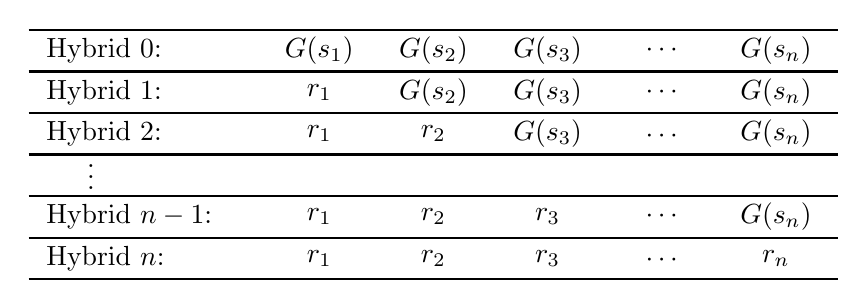
\begin{tikzpicture}[x=0.75pt,y=0.75pt,yscale=-1,xscale=1]
%uncomment if require: \path (0,300); %set diagram left start at 0, and has height of 300

%Straight Lines [id:da6691560220286636] 
\draw    (0,0) -- (390,0) ;
%Straight Lines [id:da14937141719479574] 
\draw    (0,20) -- (390,20) ;
%Straight Lines [id:da19416400836028047] 
\draw    (0,40) -- (390,40) ;
%Straight Lines [id:da4673631663401927] 
\draw    (0,60) -- (390,60) ;
%Straight Lines [id:da20994958717605572] 
\draw    (0,80) -- (390,80) ;
%Straight Lines [id:da07444150912485936] 
\draw    (0,100) -- (390,100) ;
%Straight Lines [id:da5538446859570711] 
\draw    (0,120) -- (390,120) ;

% Text Node
\draw (7,10) node [anchor=west] [inner sep=0.75pt]   [align=left] {Hybrid $\displaystyle 0$:};
% Text Node
\draw (7,30) node [anchor=west] [inner sep=0.75pt]   [align=left] {Hybrid $\displaystyle 1$:};
% Text Node
\draw (7,50) node [anchor=west] [inner sep=0.75pt]   [align=left] {Hybrid $\displaystyle 2$:};
% Text Node
\draw (7,90) node [anchor=west] [inner sep=0.75pt]   [align=left] {Hybrid $\displaystyle n-1$:};
% Text Node
\draw (7,110) node [anchor=west] [inner sep=0.75pt]   [align=left] {Hybrid $\displaystyle n$:};
% Text Node
\draw (140,10) node    {$G( s_{1})$};
% Text Node
\draw (195,10) node    {$G( s_{2})$};
% Text Node
\draw (250,10) node    {$G( s_{3})$};
% Text Node
\draw (305,10) node    {$\cdots $};
% Text Node
\draw (360,10) node    {$G( s_{n})$};
% Text Node
\draw (140,30) node    {$r_{1}$};
% Text Node
\draw (140,50) node    {$r_{1}$};
% Text Node
\draw (140,90) node    {$r_{1}$};
% Text Node
\draw (140,110) node    {$r_{1}$};
% Text Node
\draw (195,30) node    {$G( s_{2})$};
% Text Node
\draw (250,30) node    {$G( s_{3})$};
% Text Node
\draw (250,50) node    {$G( s_{3})$};
% Text Node
\draw (305,30) node    {$\cdots $};
% Text Node
\draw (305,51.2) node    {$\cdots $};
% Text Node
\draw (305,90) node    {$\cdots $};
% Text Node
\draw (305,111.2) node    {$\cdots $};
% Text Node
\draw (360,30) node    {$G( s_{n})$};
% Text Node
\draw (360,50) node    {$G( s_{n})$};
% Text Node
\draw (360,90) node    {$G( s_{n})$};
% Text Node
\draw (195,50) node    {$r_{2}$};
% Text Node
\draw (195,90) node    {$r_{2}$};
% Text Node
\draw (195,110) node    {$r_{2}$};
% Text Node
\draw (250,90) node    {$r_{3}$};
% Text Node
\draw (250,110) node    {$r_{3}$};
% Text Node
\draw (360,110) node    {$r_{n}$};
% Text Node
\draw (30,67) node    {$\vdots $};


\end{tikzpicture}
	\caption{挑战者在混合$0,1,\dots,n$中准备的数值。每个$r_i$都是$\mathcal{R}$上的一个随机元素,每个$s_i$都是$\mathcal{S}$上的一个随机元素。}
	\label{fig:3-5}
\end{figure}

接下来,我们定义一个 PRG 对手 $\mathcal B$,它就 $G$ 进行攻击游戏 \ref{game:3-1},其工作方式如下:

\vspace*{10pt}

\hspace*{5pt} 当从它的挑战者处收到 $r\in\mathcal R$ 时,$\mathcal B$ 扮演 $\mathcal A$ 的挑战者的角色:

\vspace*{5pt}

\hspace*{28.5pt} 随机选取 $\omega\overset{\rm R}\leftarrow\{1,\dots,n\}$\\
\hspace*{50pt} 随机选取 $r_1\overset{\rm R}\leftarrow\mathcal R$\\
\hspace*{74pt} $\vdots$\\
\hspace*{50pt} 随机选取 $r_{\omega-1}\overset{\rm R}\leftarrow\mathcal R$\\
\hspace*{50pt} 令 $r_{\omega}\leftarrow r$\\
\hspace*{50pt} 随机选取 $s_{\omega+1}\overset{\rm R}\leftarrow\mathcal{S}$,令 $r_{\omega+1}\leftarrow G(s_{\omega+1})$\\
\hspace*{74pt} $\vdots$\\
\hspace*{50pt} 随机选取 $s_{n}\overset{\rm R}\leftarrow\mathcal{S}$,令 $r_{n}\leftarrow G(s_{j+1})$\\
\hspace*{50pt} 将 $(r_1,\dots,r_n)$ 发送给 $\mathcal A$。

\vspace*{5pt}

\hspace*{5pt} 最后,$\mathcal A$ 输出什么,$\mathcal B$ 就输出什么。

\vspace*{10pt}

令 $W_0$ 是 $\mathcal B$ 在攻击游戏 \ref{game:3-1} 的实验 $0$ 中输出 $1$ 的事件,$W_1$ 是 $\mathcal B$ 在攻击游戏 \ref{game:3-1} 的实验 $1$ 中输出 $1$ 的事件。一个关键的观察是:

\begin{quote}
\emph{对于每个固定的 $j=1,\dots,n$,当以 $\omega=j$ 为条件时,$\mathcal B$ 的攻击游戏的实验 $0$ 就相当于混合 $j-1$,而 $\mathcal B$ 的攻击游戏的实验 $1$ 就相当于混合 $j$。
}
\end{quote}
因此:
\[
\Pr[W_0\,|\,\omega=j]=p_{j-1},\quad
\Pr[W_1\,|\,\omega=j]=p_{j}
\]
所以,我们有:
\[
\Pr[W_0]
=\sum_{j=1}^n\Pr[W_0\,|\,\omega=j]\cdot\Pr[\omega=j]
=\frac{1}{n}\sum_{j=1}^n\Pr[W_0\,|\,\omega=j]
=\frac{1}{n}\sum_{j=1}^np_{j-1}
\]
类似地:
\[
\Pr[W_1]
=\sum_{j=1}^n\Pr[W_1\,|\,\omega=j]\cdot\Pr[\omega=j]
=\frac{1}{n}\sum_{j=1}^n\Pr[W_1\,|\,\omega=j]
=\frac{1}{n}\sum_{j=1}^np_{j}
\]
最终,我们有:
\[
\begin{aligned}
\mathrm{PRG}\mathsf{adv}[\mathcal{B},G]
&=|\Pr[W_1]-\Pr[W_0]|\\
&=\Bigg\lvert\frac{1}{n}\sum_{j=1}^np_j-\frac{1}{n}\sum_{j=1}^np_{j-1}\Bigg\rvert\\
&=\frac{1}{n}|p_n-p_0|
\end{aligned}
\]
将其与式 \ref{eq:3-9} 相结合,我们可以得到:
\[
\mathrm{PRG}\mathsf{adv}[\mathcal{A},G']
=n\cdot
\mathrm{PRG}\mathsf{adv}[\mathcal{B},G]
\]
由于我们假设 $G$ 是一个安全的 PRG,因此 ${\rm PRG\mathsf{adv}}[\mathcal{B},G]$ 可忽略不计,而由于 $n$ 是多项式边界的,$\mathrm{PRG}\mathsf{adv}[\mathcal{B},G']$ 就也是可忽略不计的(见事实 \ref{fact:2-6})。这就证明了该定理。
\end{proof}

定理 \ref{theo:3-2} 表明,PRG 的安全性随着我们使用它的次数增多而最多呈线性下降。有人可能会问,这个约束是否是严格的?也即,安全性是否真的会随着使用次数的增加而线性下降?答案其实是肯定的(见练习 \ref{exer:3-14})。

\subsection{一种串行构造:Blum-Micali 方法}\label{subsec:3-4-2}

我们下面介绍一种由 Blum 和 Micali 发明的串行构造,它使用一个只能稍微拉伸一点的 PRG 来构建一个可以拉伸到任意长度的 PRG。

令 $G$ 是一个定义在 $(\mathcal{S},\mathcal{R}\times\mathcal{S})$ 上的 PRG,其中 $\mathcal S$ 和 $\mathcal R$ 是两个有限集。对于每个多项式边界的值 $n\geq 1$,我们都可以构造一个定义在 $(\mathcal{S},\mathcal{R}^n\times\mathcal{S})$ 上的新 PRG $G'$。对于 $s\in\mathcal{S}$,我们令:

\vspace*{10pt}

\hspace*{5pt} $G'(s):=$\\
\hspace*{50pt} $s_0\leftarrow s$\\
\hspace*{50pt} 对于 $i\leftarrow1$ 到 $n$:\\
\hspace*{75pt} 令 $(r_i,s_i)\leftarrow G(s_{i-1})$\\
\hspace*{50pt} 输出 $(r_1,\dots,r_n,s_n)$

\vspace*{10pt}

\noindent
我们称 $G'$ 为 \textbf{$G$ 的 $n$ 次串行组合 ($n$-wise sequential composition of $G$)}。图 \ref{fig:3-6} 是 $n=3$ 时$G'$ 的示意图。

\begin{figure}
	\centering
	\tikzset{every picture/.style={line width=0.75pt}}

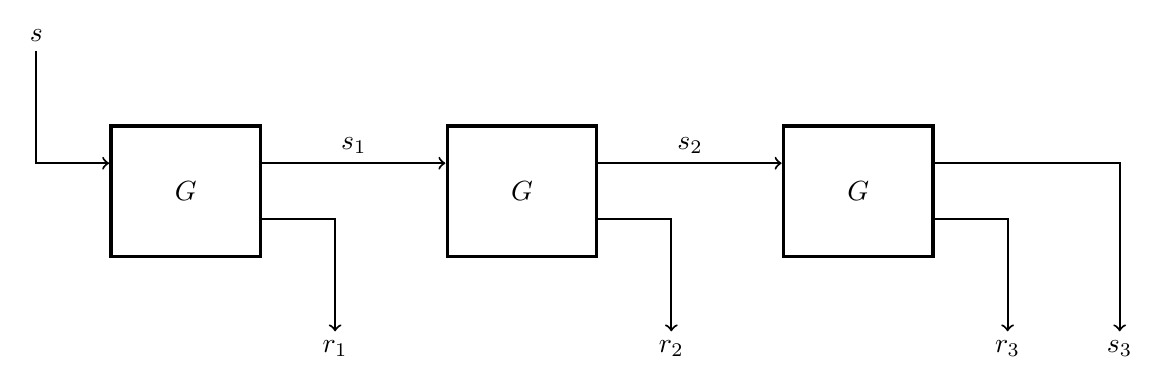
\begin{tikzpicture}[x=0.75pt,y=0.75pt,yscale=-0.9,xscale=0.9]

\draw  [line width=1.2]  (60,40) -- (140,40) -- (140,110) -- (60,110) -- cycle ;
\draw  [line width=1.2]  (240,40) -- (320,40) -- (320,110) -- (240,110) -- cycle ;
\draw  [line width=1.2]  (420,40) -- (500,40) -- (500,110) -- (420,110) -- cycle ;

\draw  [->]  (20,0) -- (20,60) -- (59,60) ;
\draw  [->]  (140,60) -- (239,60) ;
\draw  [->]  (320,60) -- (419,60) ;
\draw  [->]  (500,60) -- (600,60) -- (600,150) ;
\draw  [->]  (140,90) -- (180,90) -- (180,150) ;
\draw  [->]  (320,90) -- (360,90) -- (360,150) ;
\draw  [->]  (500,90) -- (540,90) -- (540,150) ;

\draw (20,-3.4) node [anchor=south] [inner sep=0.75pt]    {$s$};
\draw (100,75) node    {$G$};
\draw (280,75) node    {$G$};
\draw (460,75) node    {$G$};
\draw (190,56.6) node [anchor=south] [inner sep=0.75pt]    {$s_{1}$};
\draw (370,56.6) node [anchor=south] [inner sep=0.75pt]    {$s_{2}$};
\draw (180,153.4) node [anchor=north] [inner sep=0.75pt]    {$r_{1}$};
\draw (360,153.4) node [anchor=north] [inner sep=0.75pt]    {$r_{2}$};
\draw (540,153.4) node [anchor=north] [inner sep=0.75pt]    {$r_{3}$};
\draw (600,153.4) node [anchor=north] [inner sep=0.75pt]    {$s_{3}$};


\end{tikzpicture}
	\caption{$n=3$时的串行构造}
	\label{fig:3-6}
\end{figure}

我们将在下面的定理 \ref{theo:3-3} 中证明,如果 $G$ 是一个安全的 PRG,则 $G'$ 也是一个安全的 PRG。作为这个构造的一个特例,假设 $G$ 是一个定义在 $(\{0,1\}^\ell,\{0,1\}^{t+\ell})$ 上的 PRG,其中 $\ell$ 和 $t$ 都是正整数;也就是说,$G$ 把 $\ell$ 比特的序列拉伸为 $t+\ell$ 比特的序列。我们可以很自然地把 $G$ 的输出空间看作是 $\{0,1\}^t\times\{0,1\}^\ell$。应用上述构造,并将输出视作比特序列,我们就能得到一个PRG $G'$,它能把 $\ell$ 比特的序列拉伸为 $nt+\ell$ 比特的序列。

\begin{theorem}\label{theo:3-3}
如果 $G$ 是一个安全的 PRG,则 $G$ 的 $n$ 次串行组合 $G'$ 也是一个安全的 PRG。
\begin{quote}
特别地,对于每个就 $G'$ 进行攻击游戏 \ref{game:3-1} 的 PRG 对手 $\mathcal A$,都存在一个就 $G$ 进行攻击游戏 \ref{game:3-1} 的 PRG 对手 $\mathcal B$,其中 $\mathcal B$ 是一个围绕 $\mathcal A$ 的基本包装器,满足:
\end{quote}
\[
\mathrm{PRG}\mathsf{adv}[\mathcal{A},G']
=n\cdot
\mathrm{PRG}\mathsf{adv}[\mathcal{B},G]
\]
\end{theorem}

\begin{proof}[证明思路]
对该定理的证明也是一个混合论证,其思路与定理 \ref{theo:3-2} 的证明非常相似。该定理基于这样的直觉:考虑一个 PRG 对手 $\mathcal A$,它在攻击游戏 \ref{game:3-1} 的实验 $0$ 中收到 $(r_1,\dots,r_n,s_n)$。由于 $s=s_0$ 是随机的,而且 $G$ 是一个安全的 PRG,我们可以用 $\mathcal{R}\times\mathcal{S}$ 中的一个完全随机的元素来代替 $(r_1,s_1)$,并且 $\mathcal A$ 在这个新的混合游戏中输出 $1$ 的概率应该只会发生可忽略不计的变化。现在,由于 $s_1$ 是随机的(同样是因为$G$ 是一个安全的 PRG),我们就可以用 $\mathcal{R}\times\mathcal{S}$ 上的一个完全随机的元素来代替 $(r_2,s_2)$,而 $\mathcal A$ 在这第二个混合游戏中输出 $1$ 的概率应该也只会发生可忽略不计的变化。继续这样下去,我们可以用 $\mathcal{R}\times\mathcal{S}$ 中的随机元素逐步替换 $(r_3,s_3)$ 到 $(r_n,s_n)$,在做出这些改变之后,$\mathcal A$ 输出 $1$ 的概率应该都只会发生可忽略不计的变化(假设 $n$ 是多项式边界的)。然而在此时,$\mathcal A$ 输出 $1$ 的概率与它在攻击游戏 \ref{game:3-1} 的实验 $1$ 中输出 $1$ 的概率是相同的。因此,这个概率与 $\mathcal A$ 在攻击游戏 \ref{game:3-1} 的实验 $0$ 中输出 $1$ 的概率极其接近,近乎可忽略不计。

这就是我们的想法。然而,就像在定理 \ref{theo:3-2} 的证明中那样,出于技术原因,我们需要设计\emph{一个}攻击 $G$ 的 PRG 对手。
\end{proof}

\begin{proof}
令 $\mathcal A$ 是一个就 $G'$ 进行攻击游戏 \ref{game:3-1} 的 PRG 对手。我们首先引入一个大小为 $n+1$ 的混合游戏序列,称为混合 $0$,混合 $1$,$\dots$,混合 $n$。对于 $j=0,1,\dots,n$,我们定义混合 $j$ 为 $\mathcal A$ 和下述挑战者之间的游戏:

\vspace*{10pt}

\hspace*{5pt} 随机选取 $r_1\overset{\rm R}\leftarrow\mathcal R$\\
\hspace*{50pt} $\vdots$\\
\hspace*{26pt} 随机选取 $r_j\overset{\rm R}\leftarrow\mathcal R$\\
\hspace*{26pt} 随机选取 $s_j\overset{\rm R}\leftarrow\mathcal S$\\
\hspace*{26pt} 令 $(r_{j+1},s_{j+1})\leftarrow G(s_{j})$\\
\hspace*{50pt} $\vdots$\\
\hspace*{26pt} 令 $(r_n,s_{n})\leftarrow G(s_{n-1})$\\
\hspace*{26pt} 将 $(r_1,\dots,r_n,s_n)$ 发送给 $\mathcal A$。

\vspace*{10pt}

\noindent
同之前一样,$\mathcal A$ 在游戏结束时输出 $0$ 或 $1$。图 \ref{fig:3-7} 展示了挑战者在 $n=3$ 的情况下的工作流程。记 $p_0$ 为 $\mathcal A$ 在混合 $j$ 中输出 $1$ 的概率。请注意,$p_0$ 也等于 $\mathcal A$ 在攻击游戏 \ref{game:3-1} 的实验 $0$ 中输出 $1$ 的概率,而 $p_n$ 等于 $\mathcal A$ 在攻击游戏 \ref{game:3-1} 的实验 $1$ 中输出 $1$ 的概率。因此,我们有:
\begin{equation}
\mathrm{PRG}\mathsf{adv}[\mathcal{A},G']
=|p_n-p_0|
\end{equation}

\begin{figure}
	\centering
	\tikzset{every picture/.style={line width=0.75pt}}

\begin{tikzpicture}[x=0.75pt,y=0.75pt,yscale=-0.9,xscale=0.9]

\draw  [line width=1.2]  (110,40) -- (190,40) -- (190,110) -- (110,110) -- cycle ;
\draw  [line width=1.2]  (290,40) -- (370,40) -- (370,110) -- (290,110) -- cycle ;
\draw  [line width=1.2]  (470,40) -- (550,40) -- (550,110) -- (470,110) -- cycle ;
\draw  [line width=1.2]  (290,210) -- (370,210) -- (370,280) -- (290,280) -- cycle ;
\draw  [line width=1.2]  (470,210) -- (550,210) -- (550,280) -- (470,280) -- cycle ;
\draw  [line width=1.2]  (470,380) -- (550,380) -- (550,450) -- (470,450) -- cycle ;

\draw   (50,60) .. controls (50,54.48) and (54.48,50) .. (60,50) .. controls (65.52,50) and (70,54.48) .. (70,60) .. controls (70,65.52) and (65.52,70) .. (60,70) .. controls (54.48,70) and (50,65.52) .. (50,60) -- cycle ;
\draw   (170,230) .. controls (170,224.48) and (174.48,220) .. (180,220) .. controls (185.52,220) and (190,224.48) .. (190,230) .. controls (190,235.52) and (185.52,240) .. (180,240) .. controls (174.48,240) and (170,235.52) .. (170,230) -- cycle ;
\draw   (350,400) .. controls (350,394.48) and (354.48,390) .. (360,390) .. controls (365.52,390) and (370,394.48) .. (370,400) .. controls (370,405.52) and (365.52,410) .. (360,410) .. controls (354.48,410) and (350,405.52) .. (350,400) -- cycle ;
\draw   (530,570) .. controls (530,564.48) and (534.48,560) .. (540,560) .. controls (545.52,560) and (550,564.48) .. (550,570) .. controls (550,575.52) and (545.52,580) .. (540,580) .. controls (534.48,580) and (530,575.52) .. (530,570) -- cycle ;
\draw   (170,260) .. controls (170,254.48) and (174.48,250) .. (180,250) .. controls (185.52,250) and (190,254.48) .. (190,260) .. controls (190,265.52) and (185.52,270) .. (180,270) .. controls (174.48,270) and (170,265.52) .. (170,260) -- cycle ;
\draw   (170,430) .. controls (170,424.48) and (174.48,420) .. (180,420) .. controls (185.52,420) and (190,424.48) .. (190,430) .. controls (190,435.52) and (185.52,440) .. (180,440) .. controls (174.48,440) and (170,435.52) .. (170,430) -- cycle ;
\draw   (350,430) .. controls (350,424.48) and (354.48,420) .. (360,420) .. controls (365.52,420) and (370,424.48) .. (370,430) .. controls (370,435.52) and (365.52,440) .. (360,440) .. controls (354.48,440) and (350,435.52) .. (350,430) -- cycle ;
\draw   (170,600) .. controls (170,594.48) and (174.48,590) .. (180,590) .. controls (185.52,590) and (190,594.48) .. (190,600) .. controls (190,605.52) and (185.52,610) .. (180,610) .. controls (174.48,610) and (170,605.52) .. (170,600) -- cycle ;
\draw   (350,600) .. controls (350,594.48) and (354.48,590) .. (360,590) .. controls (365.52,590) and (370,594.48) .. (370,600) .. controls (370,605.52) and (365.52,610) .. (360,610) .. controls (354.48,610) and (350,605.52) .. (350,600) -- cycle ;
\draw   (530,600) .. controls (530,594.48) and (534.48,590) .. (540,590) .. controls (545.52,590) and (550,594.48) .. (550,600) .. controls (550,605.52) and (545.52,610) .. (540,610) .. controls (534.48,610) and (530,605.52) .. (530,600) -- cycle ;

\draw  [->]  (70,60) -- (109,60) ;
\draw  [->]  (190,60) -- (289,60) ;
\draw  [->]  (370,60) -- (469,60) ;
\draw  [->]  (550,60) -- (650,60) -- (650,150) ;
\draw  [->]  (190,90) -- (230,90) -- (230,150) ;
\draw  [->]  (370,90) -- (410,90) -- (410,150) ;
\draw  [->]  (550,90) -- (590,90) -- (590,150) ;
\draw  [->]  (190,230) -- (289,230) ;
\draw  [->]  (370,230) -- (469,230) ;
\draw  [->]  (550,230) -- (650,230) -- (650,320) ;
\draw  [->]  (190,260) -- (230,260) -- (230,320) ;
\draw  [->]  (370,260) -- (410,260) -- (410,320) ;
\draw  [->]  (550,260) -- (590,260) -- (590,320) ;
\draw  [->]  (370,400) -- (469,400) ;
\draw  [->]  (550,400) -- (650,400) -- (650,490) ;
\draw  [->]  (190,430) -- (230,430) -- (230,490) ; 
\draw  [->]  (370,430) -- (410,430) -- (410,490) ;
\draw  [->]  (550,430) -- (590,430) -- (590,490) ;
\draw  [->]  (550,570) -- (650,570) -- (650,660) ;
\draw  [->]  (190,600) -- (230,600) -- (230,660) ;
\draw  [->]  (370,600) -- (410,600) -- (410,660) ;
\draw  [->]  (550,600) -- (590,600) -- (590,660) ;

\draw (150,75) node    {$G$};
\draw (330,75) node    {$G$};
\draw (510,75) node    {$G$};
\draw (230,153.4) node [anchor=north] [inner sep=0.75pt]    {$r_{1}$};
\draw (410,153.4) node [anchor=north] [inner sep=0.75pt]    {$r_{2}$};
\draw (590,153.4) node [anchor=north] [inner sep=0.75pt]    {$r_{3}$};
\draw (650,153.4) node [anchor=north] [inner sep=0.75pt]    {$s_{3}$};
\draw (60,60) node    {$\mathcal{S}$};
\draw (330,245) node    {$G$};
\draw (510,245) node    {$G$};
\draw (230,323.4) node [anchor=north] [inner sep=0.75pt]    {$r_{1}$};
\draw (410,323.4) node [anchor=north] [inner sep=0.75pt]    {$r_{2}$};
\draw (590,323.4) node [anchor=north] [inner sep=0.75pt]    {$r_{3}$};
\draw (650,323.4) node [anchor=north] [inner sep=0.75pt]    {$s_{3}$};
\draw (180,230) node    {$\mathcal{S}$};
\draw (510,415) node    {$G$};
\draw (230,493.4) node [anchor=north] [inner sep=0.75pt]    {$r_{1}$};
\draw (410,493.4) node [anchor=north] [inner sep=0.75pt]    {$r_{2}$};
\draw (590,493.4) node [anchor=north] [inner sep=0.75pt]    {$r_{3}$};
\draw (650,493.4) node [anchor=north] [inner sep=0.75pt]    {$s_{3}$};
\draw (360,400) node    {$\mathcal{S}$};
\draw (230,663.4) node [anchor=north] [inner sep=0.75pt]    {$r_{1}$};
\draw (410,663.4) node [anchor=north] [inner sep=0.75pt]    {$r_{2}$};
\draw (590,663.4) node [anchor=north] [inner sep=0.75pt]    {$r_{3}$};
\draw (650,663.4) node [anchor=north] [inner sep=0.75pt]    {$s_{3}$};

\draw (540,570) node    {$\mathcal{S}$};
\draw (180,260) node    {$\mathcal{R}$};
\draw (180,430) node    {$\mathcal{R}$};
\draw (360,430) node    {$\mathcal{R}$};
\draw (180,600) node    {$\mathcal{R}$};
\draw (360,600) node    {$\mathcal{R}$};
\draw (540,600) node    {$\mathcal{R}$};

\draw (7,18) node [anchor=north west][inner sep=0.75pt]   [align=left] {混合 $0$};
\draw (7,188) node [anchor=north west][inner sep=0.75pt]   [align=left] {混合 $1$};
\draw (7,358) node [anchor=north west][inner sep=0.75pt]   [align=left] {混合 $2$};
\draw (7,548) node [anchor=north west][inner sep=0.75pt]   [align=left] {混合 $3$};

\end{tikzpicture}
	\caption{$n=3$ 时,混合游戏中挑战者的计算。圆圈表示随机产生的 $\mathcal{S}$ 或 $\mathcal{R}$ 上的元素,如标签所示。}
	\label{fig:3-7}
\end{figure}

接下来,我们定义一个 PRG 对手 $\mathcal B$,它就 $G$ 进行攻击游戏 \ref{game:3-1},工作方式如下:

\vspace*{10pt}

\hspace*{5pt} 当从挑战者处收到 $(r,s)\in\mathcal{R}\times\mathcal{S}$ 时,$\mathcal B$ 扮演 $\mathcal A$ 的挑战者的角色:

\vspace*{5pt}

\hspace*{28.5pt} 随机选取 $\omega\overset{\rm R}\leftarrow\{1,\dots,n\}$\\
\hspace*{50pt} 随机选取 $r_1\overset{\rm R}\leftarrow\mathcal R,\dots,r_{\omega-1}\overset{\rm R}\leftarrow\mathcal R$\\
\hspace*{50pt} 令 $(r_{\omega},s_{\omega})\leftarrow(r,s)$\\
\hspace*{50pt} 令 $(r_{\omega+1},s_{\omega+1})\leftarrow G(s_{\omega}),\dots,(r_n,s_n)\leftarrow G(s_{n-1})$\\
\hspace*{50pt} 将 $(r_1,\dots,r_n,s_n)$ 发送给 $\mathcal A$。

\vspace*{5pt}

\hspace*{5pt} 最后,$\mathcal A$ 输出什么,$\mathcal B$ 就输出什么。

\vspace*{10pt}

令 $W_0$ 是$\mathcal B$在攻击游戏 \ref{game:3-1} 的实验 $0$ 中输出 $1$ 的事件,$W_1$ 是$\mathcal B$在攻击游戏 \ref{game:3-1} 的实验 $1$ 中输出 $1$ 的事件。一个关键的观察是:
\begin{quote}
\emph{对于每个固定的 $j=1,\dots,n$,当以 $\omega=j$ 为条件时,$\mathcal B$ 的攻击游戏的实验 $0$ 就相当于混合 $j-1$,而 $\mathcal B$ 的攻击游戏的实验 $1$ 就相当于混合 $j$。
}
\end{quote}
因此:
\[
\Pr[W_0\,|\,\omega=j]=p_{j-1},
\quad
\Pr[W_1\,|\,\omega=j]=p_{j}
\]

接下来的证明只是简单的计算,与定理 \ref{theo:3-2} 的证明的最后一段\emph{相同},不再赘述。
\end{proof}

评价 PRG 的一个标准是它的\textbf{扩展率 (expansion rate)}:一个将 $n$ 比特种子拉伸为 $m$ 比特输出的 PRG 的扩展率就是 $m/n$。更一般地说,如果种子空间是 $\mathcal{S}$,输出空间是 $\mathcal{R}$,我们就可以将扩展率定义为 $\log|\mathcal{R}|/\log|\mathcal{S}|$。串行组合能够比并行组合提供更高的扩展率,但是它有一个缺点,那就是它不能被并行化。事实上,存在一种构造可以同时兼顾高扩展率和高度可并行构造这两个优点,见 \ref{subsec:4-4-4} 小节。

\subsection{数学细节}\label{subsec:3-4-3}

在定理 \ref{theo:3-2} 和 \ref{theo:3-3} 的证明中,有一些微妙的细节值得讨论。

首先,在这两个构造中,底层的 PRG $G$ 可能包含系统参数。也就是说,可能存在一个概率性算法,它将安全参数 $\lambda$ 作为输入,并输出一个系统参数 $\Lambda$。回顾一下,系统参数是能够完全地将构造实例化的公共数据(在这个场景中,它可能定义了种子空间和输出空间)。对于并行和串行构造,我们可以对 $G$ 的所有 $n$ 个实例使用相同的系统参数;事实上,对于串行构造来说,这是必须的,因为我们要确保一轮的输出可以被用作下一轮的输入。无论是对所有 $G$ 的实例使用相同的系统参数,还是对不同的实例使用不同的系统参数,这些安全定理的证明都是完全有效的。

其次,我们简要讨论关于混合论证的一个更深刻的问题。为了更具体一点,我们把注意力集中在定理 \ref{theo:3-2} 的证明上(尽管类似的讨论也适用于定理 \ref{theo:3-3} 的证明,或任何其他的混合论证)。在证明该定理时,我们最终想要证明,如果存在一个能攻破 $G'$ 的有效对手 $\mathcal A$,那么也必然存在一个能攻破 $G$ 的有效对手。假设 $\mathcal A$ 是一个能破解 $G'$ 的有效对手,那么它相对于 $G'$ 的优势 $\epsilon(\lambda)$(我们这里明确地把它表示成安全参数 $\lambda$ 的一个函数)是不可忽略不计的。这就意味着存在一个常数 $c$ 使得 $\epsilon(\lambda)\geq{1}/{\lambda^c}$ 对无限多个 $\lambda$ 都是成立的。

现在,在定理 \ref{theo:3-2} 的证明之前的讨论中,我们考虑了 $n=2$ 的特殊情况,并表明存在有效对手 $\mathcal{B}_1$ 和 $\mathcal{B}_2$,使得 $\epsilon(\lambda)\leq\delta_1(\lambda)+\delta_2(\lambda)$ 对于任意的 $\lambda$ 都成立,其中 $\delta_j(\lambda)$ 表示 $\mathcal{B}_j$ 相对于 $G$ 的优势。由此可见,要么 $\delta_1(\lambda)\geq{1}/{2\lambda^c}$ 对无限多个 $\lambda$ 成立,要么 $\delta_2(\lambda)\geq{1}/{2\lambda^c}$ 对无限多个 $\lambda$ 成立。因此我们可以得出结论,要么是 $\mathcal{B}_1$ 攻破 $G$,要么是 $\mathcal{B}_2$ 攻破 $G$(也可能两者皆然)。因此,\emph{存在}一个能够破解 $G$ 的有效对手:它要么是 $\mathcal{B}_1$,要么就是 $\mathcal{B}_2$,我们不知道(也不必分清)到底是哪一个。然而无论是哪一个,它都是一个固定的对手,对于所有的 $\lambda$,其定义都是统一的;也就是说,它是一个固定的,以 $\lambda$ 为输入的机器。

这个论证是完全有效的,并且可以扩展到任意\emph{常数} $n$ 的情况:我们可以构造 $n$ 个对手 $\mathcal{B}_1,\dots,\mathcal{B}_n$,并论证对于某个 $j\in\{1,\dots,n\}$,对手 $\mathcal{B}_j$ 相对于 $G$ 有优势 $1/n\lambda^c$,且它对无限多个 $\lambda$ 都成立,因而能够攻破 $G$。然而这个论证并没有扩展到 $n$ 是 $\lambda$ 的一个函数的情况,我们把这种情况明确地表示成 $n(\lambda)$。问题不在于 $1/(n(\lambda)\lambda^c)$ 也许太小(其实并不是)。这个问题相当微妙,所以在讨论它之前,让我们先回顾一下我们所给出的(合法)证明。对于每个 $\lambda$,我们定义了一个大小为 $n(\lambda)+1$ 的混合游戏序列,因此对于每个 $\lambda$,我们实际上都得到了一个不同的游戏序列。事实上,我们不能说存在一个单一、有限的游戏序列对所有 $\lambda$ 都有效,因为 $n(\lambda)\to\infty$。尽管如此,我们还是明确地构造了一个固定的对手 $\mathcal B$,对于所有的 $\lambda$,它的定义都是统一的;也就是说,$\mathcal B$ 是一个固定的,以 $\lambda$ 为输入的机器。我们为每个 $\lambda$ 定义的混合游戏序列都是一个数学对象,我们对其可计算性不做任何主张——它只是我们在分析 $\mathcal B$ 时所使用的一个方便的工具。

希望到现在为止,读者至少对我们试图将常数 $n$ 的论证推广到一个函数 $n(\lambda)$ 时所产生的问题有了一个直观感觉。首先,我们甚至不清楚 $n(\lambda)$ 个对手 $\mathcal{B}_1,\dots,\mathcal{B}_{n(\lambda)}$ 是什么意思:我们的对手应该是以 $\lambda$ 为输入的固定机器,而这些机器本身不应该依赖于 $\lambda$。撇开这种语言上的混乱不谈,我们对常数情况的证明只表明存在一个``对手",对于无限多的 $\lambda$ 值来说,它能以某种方式知道 $j=j(\lambda)$ 的``正确"值,以便在 $(n(\lambda)+1)$ 游戏混合论证中使用——没有一个单独的 $j$ 的常数值一定能对无限多的 $\lambda$ 有效。如果使用非统一的计算模型,我们实际上可以使这种类型的论证有意义,但我们在本文中不会采取这种方法。

当我们使用一个构建单一对手 $\mathcal B$ 的混合论证时,所有这些问题都会消失,就像我们在定理 \ref{theo:3-2} 和 \ref{theo:3-3} 的证明中所做的那样。然而,我们重申,我们在 $n=2$,或自然延伸到每一个常数 $n$ 的情况下所做的原始分析都是完全有效的。在这种情况下,我们构建了一个单一、固定的 $n+1$ 游戏序列,每个单独的游戏对所有 $\lambda$ 都是统一定义的(就像我们的安全定义中的攻击游戏一样),我们还定义了一个有限的对手集合,每个对手都是一个固定的机器。我们重申这一点,因为在后面的内容中,我们将经常构建涉及这样的有限序列游戏的证明(事实上,定理 \ref{theo:3-1} 的证明就是这种类型)。在这种情况下,每个游戏将为所有 $\lambda$ 统一定义,并被称为游戏 $0$、游戏 $1$,等等。相反,当我们进行混合论证,使用非统一的游戏序列时,我们将这些游戏表示为混合 $0$,混合 $1$ 等,以避免任何可能的混淆。